% Robert Adams CS 475

\documentclass[letterpaper,10pt]{article} %twocolumn titlepage 
\usepackage{graphicx}
\usepackage{amssymb}
\usepackage{amsmath}
\usepackage{amsthm}

\usepackage{alltt}
\usepackage{float}
\usepackage{color}
\usepackage{url}

\usepackage{balance}
\usepackage[TABBOTCAP, tight]{subfigure}
\usepackage{enumitem}
\usepackage{pstricks, pst-node}


\usepackage{geometry}
\geometry{margin=1in, textheight=8.5in} %textwidth=6in

%random comment

\newcommand{\cred}[1]{{\color{red}#1}}
\newcommand{\cblue}[1]{{\color{blue}#1}}

\usepackage{hyperref}

\def\name{Robert Adams}
%% The following metadata will show up in the PDF properties
\hypersetup{
	colorlinks = true,
	urlcolor = black,
	pdfauthor = {\name},
	pdfkeywords = {cs745},
	pdftitle = 	{CS 475 Project 7: Functional Decomposition},
pdfsubject = {CS 475 Project 7},
	pdfpagemode = UseNone,
}


\begin{document}
\title{CS 475 Project 7: Functional Decomposition} 
\author{Robert Adams}
\maketitle



\section{Commentary}

	Height of the grain is dependent on the temperature and precipitation and the number of deer are dependent of the height of the grain.  I’ve added another factor, Exodus 7:14-25, water to blood, which has a 1 in 15 chance of occurring and when it does sets precipitation to zero for three days, killing a random number of deer each day this phenomena occurs. 

\begin{figure} [h]
	\centering
	% GNUPLOT: LaTeX picture with Postscript
\begingroup
  \makeatletter
  \providecommand\color[2][]{%
    \GenericError{(gnuplot) \space\space\space\@spaces}{%
      Package color not loaded in conjunction with
      terminal option `colourtext'%
    }{See the gnuplot documentation for explanation.%
    }{Either use 'blacktext' in gnuplot or load the package
      color.sty in LaTeX.}%
    \renewcommand\color[2][]{}%
  }%
  \providecommand\includegraphics[2][]{%
    \GenericError{(gnuplot) \space\space\space\@spaces}{%
      Package graphicx or graphics not loaded%
    }{See the gnuplot documentation for explanation.%
    }{The gnuplot epslatex terminal needs graphicx.sty or graphics.sty.}%
    \renewcommand\includegraphics[2][]{}%
  }%
  \providecommand\rotatebox[2]{#2}%
  \@ifundefined{ifGPcolor}{%
    \newif\ifGPcolor
    \GPcolorfalse
  }{}%
  \@ifundefined{ifGPblacktext}{%
    \newif\ifGPblacktext
    \GPblacktexttrue
  }{}%
  % define a \g@addto@macro without @ in the name:
  \let\gplgaddtomacro\g@addto@macro
  % define empty templates for all commands taking text:
  \gdef\gplbacktext{}%
  \gdef\gplfronttext{}%
  \makeatother
  \ifGPblacktext
    % no textcolor at all
    \def\colorrgb#1{}%
    \def\colorgray#1{}%
  \else
    % gray or color?
    \ifGPcolor
      \def\colorrgb#1{\color[rgb]{#1}}%
      \def\colorgray#1{\color[gray]{#1}}%
      \expandafter\def\csname LTw\endcsname{\color{white}}%
      \expandafter\def\csname LTb\endcsname{\color{black}}%
      \expandafter\def\csname LTa\endcsname{\color{black}}%
      \expandafter\def\csname LT0\endcsname{\color[rgb]{1,0,0}}%
      \expandafter\def\csname LT1\endcsname{\color[rgb]{0,1,0}}%
      \expandafter\def\csname LT2\endcsname{\color[rgb]{0,0,1}}%
      \expandafter\def\csname LT3\endcsname{\color[rgb]{1,0,1}}%
      \expandafter\def\csname LT4\endcsname{\color[rgb]{0,1,1}}%
      \expandafter\def\csname LT5\endcsname{\color[rgb]{1,1,0}}%
      \expandafter\def\csname LT6\endcsname{\color[rgb]{0,0,0}}%
      \expandafter\def\csname LT7\endcsname{\color[rgb]{1,0.3,0}}%
      \expandafter\def\csname LT8\endcsname{\color[rgb]{0.5,0.5,0.5}}%
    \else
      % gray
      \def\colorrgb#1{\color{black}}%
      \def\colorgray#1{\color[gray]{#1}}%
      \expandafter\def\csname LTw\endcsname{\color{white}}%
      \expandafter\def\csname LTb\endcsname{\color{black}}%
      \expandafter\def\csname LTa\endcsname{\color{black}}%
      \expandafter\def\csname LT0\endcsname{\color{black}}%
      \expandafter\def\csname LT1\endcsname{\color{black}}%
      \expandafter\def\csname LT2\endcsname{\color{black}}%
      \expandafter\def\csname LT3\endcsname{\color{black}}%
      \expandafter\def\csname LT4\endcsname{\color{black}}%
      \expandafter\def\csname LT5\endcsname{\color{black}}%
      \expandafter\def\csname LT6\endcsname{\color{black}}%
      \expandafter\def\csname LT7\endcsname{\color{black}}%
      \expandafter\def\csname LT8\endcsname{\color{black}}%
    \fi
  \fi
  \setlength{\unitlength}{0.0500bp}%
  \begin{picture}(9792.00,5040.00)%
    \gplgaddtomacro\gplbacktext{%
      \csname LTb\endcsname%
      \put(1210,744){\makebox(0,0)[r]{\strut{} 0}}%
      \put(1210,1551){\makebox(0,0)[r]{\strut{} 100}}%
      \put(1210,2357){\makebox(0,0)[r]{\strut{} 200}}%
      \put(1210,3163){\makebox(0,0)[r]{\strut{} 300}}%
      \put(1210,3970){\makebox(0,0)[r]{\strut{} 400}}%
      \put(1210,4776){\makebox(0,0)[r]{\strut{} 500}}%
      \put(1342,484){\makebox(0,0){\strut{} 0}}%
      \put(2465,484){\makebox(0,0){\strut{} 500000}}%
      \put(3588,484){\makebox(0,0){\strut{} 1e+06}}%
      \put(4711,484){\makebox(0,0){\strut{} 1.5e+06}}%
      \put(5833,484){\makebox(0,0){\strut{} 2e+06}}%
      \put(6956,484){\makebox(0,0){\strut{} 2.5e+06}}%
      \put(8079,484){\makebox(0,0){\strut{} 3e+06}}%
      \put(440,2740){\rotatebox{90}{\makebox(0,0){\strut{}GFLOPS/sec}}}%
      \put(4710,154){\makebox(0,0){\strut{}Global Size}}%
    }%
    \gplgaddtomacro\gplfronttext{%
      \csname LTb\endcsname%
      \put(8805,4666){\makebox(0,0)[r]{\strut{}1}}%
      \csname LTb\endcsname%
      \put(8805,4446){\makebox(0,0)[r]{\strut{}2}}%
      \csname LTb\endcsname%
      \put(8805,4226){\makebox(0,0)[r]{\strut{}4}}%
      \csname LTb\endcsname%
      \put(8805,4006){\makebox(0,0)[r]{\strut{}8}}%
      \csname LTb\endcsname%
      \put(8805,3786){\makebox(0,0)[r]{\strut{}16}}%
      \csname LTb\endcsname%
      \put(8805,3566){\makebox(0,0)[r]{\strut{}32}}%
      \csname LTb\endcsname%
      \put(8805,3346){\makebox(0,0)[r]{\strut{}64}}%
      \csname LTb\endcsname%
      \put(8805,3126){\makebox(0,0)[r]{\strut{}128}}%
      \csname LTb\endcsname%
      \put(8805,2906){\makebox(0,0)[r]{\strut{}256}}%
      \csname LTb\endcsname%
      \put(8805,2686){\makebox(0,0)[r]{\strut{}512}}%
      \csname LTb\endcsname%
      \put(8805,2466){\makebox(0,0)[r]{\strut{}1024}}%
      \csname LTb\endcsname%
      \put(8805,2246){\makebox(0,0)[r]{\strut{}SIMD}}%
    }%
    \gplbacktext
    \put(0,0){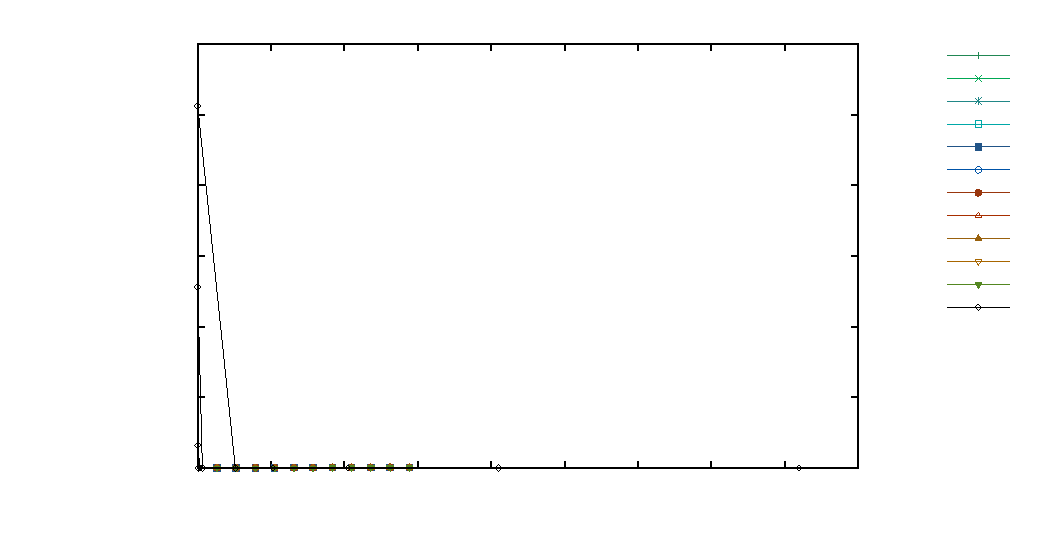
\includegraphics{global}}%
    \gplfronttext
  \end{picture}%
\endgroup

	%\caption{Speed of height calculations performed on a subdivided surface} 
	\label{runtimes}
\end{figure}

\begin{figure} [h]
	\centering
	% GNUPLOT: LaTeX picture with Postscript
\begingroup
  \makeatletter
  \providecommand\color[2][]{%
    \GenericError{(gnuplot) \space\space\space\@spaces}{%
      Package color not loaded in conjunction with
      terminal option `colourtext'%
    }{See the gnuplot documentation for explanation.%
    }{Either use 'blacktext' in gnuplot or load the package
      color.sty in LaTeX.}%
    \renewcommand\color[2][]{}%
  }%
  \providecommand\includegraphics[2][]{%
    \GenericError{(gnuplot) \space\space\space\@spaces}{%
      Package graphicx or graphics not loaded%
    }{See the gnuplot documentation for explanation.%
    }{The gnuplot epslatex terminal needs graphicx.sty or graphics.sty.}%
    \renewcommand\includegraphics[2][]{}%
  }%
  \providecommand\rotatebox[2]{#2}%
  \@ifundefined{ifGPcolor}{%
    \newif\ifGPcolor
    \GPcolorfalse
  }{}%
  \@ifundefined{ifGPblacktext}{%
    \newif\ifGPblacktext
    \GPblacktexttrue
  }{}%
  % define a \g@addto@macro without @ in the name:
  \let\gplgaddtomacro\g@addto@macro
  % define empty templates for all commands taking text:
  \gdef\gplbacktext{}%
  \gdef\gplfronttext{}%
  \makeatother
  \ifGPblacktext
    % no textcolor at all
    \def\colorrgb#1{}%
    \def\colorgray#1{}%
  \else
    % gray or color?
    \ifGPcolor
      \def\colorrgb#1{\color[rgb]{#1}}%
      \def\colorgray#1{\color[gray]{#1}}%
      \expandafter\def\csname LTw\endcsname{\color{white}}%
      \expandafter\def\csname LTb\endcsname{\color{black}}%
      \expandafter\def\csname LTa\endcsname{\color{black}}%
      \expandafter\def\csname LT0\endcsname{\color[rgb]{1,0,0}}%
      \expandafter\def\csname LT1\endcsname{\color[rgb]{0,1,0}}%
      \expandafter\def\csname LT2\endcsname{\color[rgb]{0,0,1}}%
      \expandafter\def\csname LT3\endcsname{\color[rgb]{1,0,1}}%
      \expandafter\def\csname LT4\endcsname{\color[rgb]{0,1,1}}%
      \expandafter\def\csname LT5\endcsname{\color[rgb]{1,1,0}}%
      \expandafter\def\csname LT6\endcsname{\color[rgb]{0,0,0}}%
      \expandafter\def\csname LT7\endcsname{\color[rgb]{1,0.3,0}}%
      \expandafter\def\csname LT8\endcsname{\color[rgb]{0.5,0.5,0.5}}%
    \else
      % gray
      \def\colorrgb#1{\color{black}}%
      \def\colorgray#1{\color[gray]{#1}}%
      \expandafter\def\csname LTw\endcsname{\color{white}}%
      \expandafter\def\csname LTb\endcsname{\color{black}}%
      \expandafter\def\csname LTa\endcsname{\color{black}}%
      \expandafter\def\csname LT0\endcsname{\color{black}}%
      \expandafter\def\csname LT1\endcsname{\color{black}}%
      \expandafter\def\csname LT2\endcsname{\color{black}}%
      \expandafter\def\csname LT3\endcsname{\color{black}}%
      \expandafter\def\csname LT4\endcsname{\color{black}}%
      \expandafter\def\csname LT5\endcsname{\color{black}}%
      \expandafter\def\csname LT6\endcsname{\color{black}}%
      \expandafter\def\csname LT7\endcsname{\color{black}}%
      \expandafter\def\csname LT8\endcsname{\color{black}}%
    \fi
  \fi
  \setlength{\unitlength}{0.0500bp}%
  \begin{picture}(9792.00,5040.00)%
    \gplgaddtomacro\gplbacktext{%
      \csname LTb\endcsname%
      \put(990,704){\makebox(0,0)[r]{\strut{} 0}}%
      \put(990,1111){\makebox(0,0)[r]{\strut{} 50}}%
      \put(990,1518){\makebox(0,0)[r]{\strut{} 100}}%
      \put(990,1926){\makebox(0,0)[r]{\strut{} 150}}%
      \put(990,2333){\makebox(0,0)[r]{\strut{} 200}}%
      \put(990,2740){\makebox(0,0)[r]{\strut{} 250}}%
      \put(990,3147){\makebox(0,0)[r]{\strut{} 300}}%
      \put(990,3554){\makebox(0,0)[r]{\strut{} 350}}%
      \put(990,3962){\makebox(0,0)[r]{\strut{} 400}}%
      \put(990,4369){\makebox(0,0)[r]{\strut{} 450}}%
      \put(990,4776){\makebox(0,0)[r]{\strut{} 500}}%
      \put(1122,484){\makebox(0,0){\strut{} 0}}%
      \put(2216,484){\makebox(0,0){\strut{} 200}}%
      \put(3309,484){\makebox(0,0){\strut{} 400}}%
      \put(4403,484){\makebox(0,0){\strut{} 600}}%
      \put(5496,484){\makebox(0,0){\strut{} 800}}%
      \put(6590,484){\makebox(0,0){\strut{} 1000}}%
      \put(7683,484){\makebox(0,0){\strut{} 1200}}%
      \put(4402,154){\makebox(0,0){\strut{}Local Size}}%
    }%
    \gplgaddtomacro\gplfronttext{%
      \csname LTb\endcsname%
      \put(8805,4666){\makebox(0,0)[r]{\strut{}262144}}%
      \csname LTb\endcsname%
      \put(8805,4446){\makebox(0,0)[r]{\strut{}524288}}%
      \csname LTb\endcsname%
      \put(8805,4226){\makebox(0,0)[r]{\strut{}786432}}%
      \csname LTb\endcsname%
      \put(8805,4006){\makebox(0,0)[r]{\strut{}1048576}}%
      \csname LTb\endcsname%
      \put(8805,3786){\makebox(0,0)[r]{\strut{}1310720}}%
      \csname LTb\endcsname%
      \put(8805,3566){\makebox(0,0)[r]{\strut{}1572864}}%
      \csname LTb\endcsname%
      \put(8805,3346){\makebox(0,0)[r]{\strut{}1835008}}%
      \csname LTb\endcsname%
      \put(8805,3126){\makebox(0,0)[r]{\strut{}2097152}}%
      \csname LTb\endcsname%
      \put(8805,2906){\makebox(0,0)[r]{\strut{}2359296}}%
      \csname LTb\endcsname%
      \put(8805,2686){\makebox(0,0)[r]{\strut{}2621440}}%
      \csname LTb\endcsname%
      \put(8805,2466){\makebox(0,0)[r]{\strut{}2883584}}%
    }%
    \gplbacktext
    \put(0,0){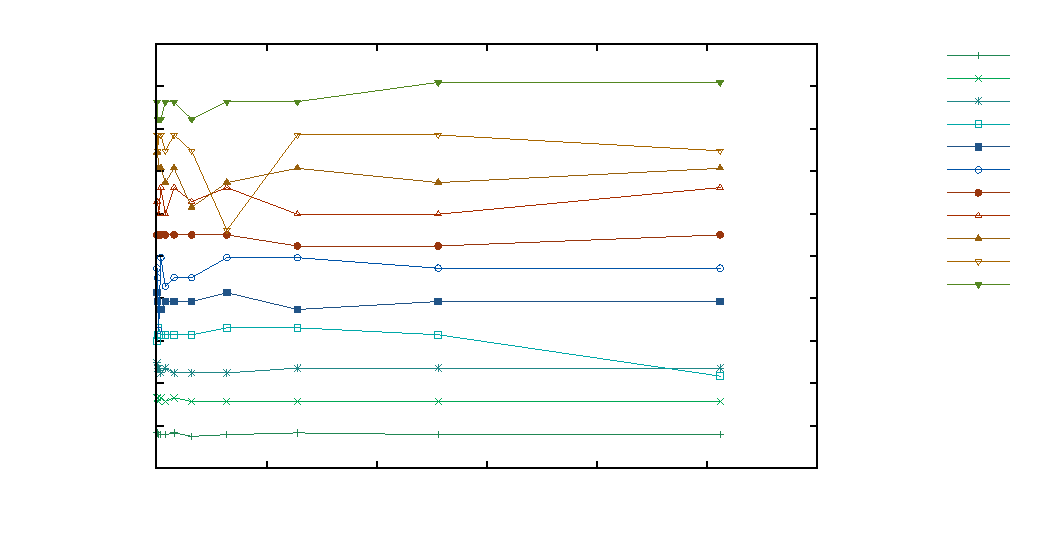
\includegraphics{local}}%
    \gplfronttext
  \end{picture}%
\endgroup

	%\caption{Speed of height calculations performed on a subdivided surface} 
	\label{runtimes}
\end{figure}

\begin{table}  [ht]
	\centering
	    \begin{tabular}{llllll}
\verb|#|months & precipitation, in. & temperature, celsuis & height, in.
               & \#deer & blood rain\\ \hline 
0 & 7.130446 & 3.047354 & 7.280658 & 1 & 0\\ 
1 & 11.88923 & 5.459258 & 7.399446 & 2 & 0\\ 
2 & 12.868473 & 5.293376 & 7.097805 & 3 & 0\\ 
3 & 11.705143 & 13.475433 & 0 & 4 & 0\\ 
4 & 0 & 16.354347 & 0.090767 & 0 & 3\\ 
5 & 0 & 22.240419 & 0 & 0 & 2\\ 
6 & 0 & 15.358073 & 0.123071 & 0 & 1\\ 
7 & 1.361137 & 14.042067 & 0 & 1 & 0\\ 
8 & 2.200143 & 8.529198 & 2.852644 & 0 & 0\\ 
9 & 1.560894 & 7.267927 & 2.910112 & 1 & 0\\ 
10 & 2.307568 & -0.123056 & 2.033391 & 2 & 0\\ 
11 & 6.338187 & -0.80381 & 1.724264 & 3 & 0\\ 
12 & 7.659895 & 2.282577 & 6.323122 & 2 & 0\\ 
13 & 9.119032 & -1.84108 & 0.982858 & 3 & 0\\ 
14 & 11.473538 & 0.503907 & 4.324983 & 2 & 0\\ 
15 & 13.592863 & 2.343737 & 5.85623 & 3 & 0\\ 
16 & 10.56441 & 8.276389 & 4.074954 & 4 & 0\\ 
17 & 9.638212 & 22.192663 & 0 & 5 & 0\\ 
18 & 7.383721 & 15.399433 & 0 & 4 & 0\\ 
19 & 6.329622 & 17.824512 & 0 & 3 & 0\\ 
20 & 0.824023 & 21.755852 & 0 & 2 & 0\\ 
21 & 1.24544 & 11.489178 & 0.337651 & 1 & 0\\ 
22 & 0.330871 & 8.98783 & 1.810299 & 0 & 0\\ 
23 & 3.484699 & 1.450344 & 3.902967 & 1 & 0\\ 
24 & 3.58426 & 1.722516 & 3.690594 & 2 & 0\\ 
25 & 6.96911 & 0.822811 & 3.867681 & 3 & 0\\ 
26 & 7.313332 & -4.443907 & 0 & 4 & 0\\ 
27 & 9.563989 & 5.801049 & 6.96293 & 3 & 0\\ 
28 & 11.196996 & 11.49504 & 0 & 4 & 0\\ 
29 & 12.150116 & 17.947634 & 0 & 3 & 0\\ 
30 & 10.00088 & 21.842033 & 0 & 2 & 0\\ 
31 & 8.811982 & 19.604031 & 0 & 1 & 0\\ 
32 & 4.377048 & 25.29887 & 0.000005 & 0 & 0\\ 
33 & 3.437872 & 22.859549 & 0.000099 & 1 & 0\\ 
34 & 0.768767 & 17.109791 & 0.021232 & 0 & 0\\ 
35 & 0 & 8.453083 & 1.967145 & 1 & 0\\ 
36 & 1.545493 & 0.003904 & 1.324631 & 2 & 0\\ 
37 & 3.552026 & -4.204365 & 0.026175 & 1 & 0\\ 
38 & 6.231343 & -1.660273 & 1.834336 & 0 & 0\\ 
39 & 6.057216 & -5.141718 & 0 & 1 & 0\\ 
40 & 12.181647 & 5.037426 & 8.484457 & 0 & 0\\ 
41 & 11.328308 & 9.173622 & 3.784272 & 1 & 0\\ 
42 & 10.972197 & 11.416474 & 1.345657 & 2 & 0\\ 
43 & 9.220291 & 18.795506 & 0 & 1 & 0\\ 
44 & 6.054814 & 23.311937 & 0.000075 & 0 & 0\\ 
45 & 5.427371 & 17.000311 & 0.04417 & 1 & 0\\ 
46 & 0 & 22.857901 & 0 & 0 & 0\\ 
47 & 0 & 9.278107 & 1.553051 & 0 & 0\\ 
48 & 0 & 9.709282 & 1.081516 & 0 & 3\\ 
49 & 0 & 5.029204 & 2.860969 & 0 & 2\\ 
50 & 0 & -5.41882 & 0.226778 & 0 & 1\\ 
51 & 7.846189 & 2.81946 & 7.387514 & 1 & 0\\ 
52 & 0 & -5.710967 & 0 & 2 & 3\\ 
53 & 0 & 6.476098 & 7.250269 & 1 & 3\\ 
54 & 0 & 11.241343 & 2.014443 & 0 & 2\\ 
55 & 0 & 13.919013 & 0.489724 & 0 & 1\\ 

		    \end{tabular}
	\end{table}

	\end{document}
